\chapter{Технологический раздел}
\label{cha:technological}

    В данном разделе представлены результаты анкетирования, построена функция принадлежности, представлены средства, использованные в процессе разработки для реализации задачи, а также листинг кода программы. Кроме того показаны результаты тестирования.

    \section{Результаты анкетирования}
    \par В таблице \ref{tab:anket2} представлены результаты анкетирования 5-ти респондентов. Заполнение анкет выполнялось по бинарному признаку: «1» ставилась там, где утверждение считалось респондентами верным, и «0» там, где нет соответственно.
    \begin{table}[!h]
    \centering
    \caption{Результаты анкетирования}
\begin{tabular}{|l|l|l|l|l|l|l|l|l|l|l|l|l|}
\hline
                          &                 & 0 & 5 & 10 & 15 & 20 & 25 & 30 & 35 & 40 & 45 & 50 \\ \hline
\multirow{6}{*}{Карина}   & очень маленький & 1 & 1 & 0  & 0  & 0  & 0  & 0  & 0  & 0  & 0  & 0  \\ \cline{2-13} 
                          & маленький       & 0 & 0 & 1  & 1  & 0  & 0  & 0  & 0  & 0  & 0  & 0  \\ \cline{2-13} 
                          & небольшой       & 0 & 0 & 0  & 0  & 1  & 1  & 0  & 0  & 0  & 0  & 0  \\ \cline{2-13} 
                          & средний         & 0 & 0 & 0  & 0  & 0  & 0  & 1  & 1  & 0  & 0  & 0  \\ \cline{2-13} 
                          & большой         & 0 & 0 & 0  & 0  & 0  & 0  & 0  & 0  & 1  & 1  & 0  \\ \cline{2-13} 
                          & очень большой   & 0 & 0 & 0  & 0  & 0  & 0  & 0  & 0  & 0  & 0  & 1  \\ \hline
\multirow{6}{*}{Вероника} & очень маленький & 1 & 1 & 0  & 0  & 0  & 0  & 0  & 0  & 0  & 0  & 0  \\ \cline{2-13} 
                          & маленький       & 0 & 0 & 1  & 0  & 0  & 0  & 0  & 0  & 0  & 0  & 0  \\ \cline{2-13} 
                          & небольшой       & 0 & 0 & 0  & 1  & 0  & 0  & 0  & 0  & 0  & 0  & 0  \\ \cline{2-13} 
                          & средний         & 0 & 0 & 0  & 0  & 1  & 1  & 1  & 0  & 0  & 0  & 0  \\ \cline{2-13} 
                          & большой         & 0 & 0 & 0  & 0  & 0  & 0  & 0  & 1  & 1  & 1  & 0  \\ \cline{2-13} 
                          & очень большой   & 0 & 0 & 0  & 0  & 0  & 0  & 0  & 0  & 0  & 0  & 1  \\ \hline
\multirow{6}{*}{Илья}     & очень маленький & 1 & 1 & 0  & 0  & 0  & 0  & 0  & 0  & 0  & 0  & 0  \\ \cline{2-13} 
                          & маленький       & 0 & 0 & 1  & 1  & 0  & 0  & 0  & 0  & 0  & 0  & 0  \\ \cline{2-13} 
                          & небольшой       & 0 & 0 & 0  & 0  & 1  & 0  & 0  & 0  & 0  & 0  & 0  \\ \cline{2-13} 
                          & средний         & 0 & 0 & 0  & 0  & 0  & 1  & 1  & 0  & 0  & 0  & 0  \\ \cline{2-13} 
                          & большой         & 0 & 0 & 0  & 0  & 0  & 0  & 0  & 1  & 1  & 1  & 0  \\ \cline{2-13} 
                          & очень большой   & 0 & 0 & 0  & 0  & 0  & 0  & 0  & 0  & 0  & 0  & 1  \\ \hline
\multirow{6}{*}{Леша}     & очень маленький & 1 & 1 & 0  & 0  & 0  & 0  & 0  & 0  & 0  & 0  & 0  \\ \cline{2-13} 
                          & маленький       & 0 & 1 & 1  & 0  & 0  & 0  & 0  & 0  & 0  & 0  & 0  \\ \cline{2-13} 
                          & небольшой       & 0 & 0 & 1  & 1  & 0  & 0  & 0  & 0  & 0  & 0  & 0  \\ \cline{2-13} 
                          & средний         & 0 & 0 & 0  & 1  & 1  & 1  & 1  & 0  & 0  & 0  & 0  \\ \cline{2-13} 
                          & большой         & 0 & 0 & 0  & 0  & 0  & 0  & 1  & 1  & 0  & 0  & 0  \\ \cline{2-13} 
                          & очень большой   & 0 & 0 & 0  & 0  & 0  & 0  & 0  & 0  & 1  & 1  & 1  \\ \hline
\multirow{6}{*}{Катя}     & очень маленький & 1 & 1 & 1  & 0  & 0  & 0  & 0  & 0  & 0  & 0  & 0  \\ \cline{2-13} 
                          & маленький       & 0 & 0 & 0  & 1  & 0  & 0  & 0  & 0  & 0  & 0  & 0  \\ \cline{2-13} 
                          & небольшой       & 0 & 0 & 0  & 0  & 1  & 0  & 0  & 0  & 0  & 0  & 0  \\ \cline{2-13} 
                          & средний         & 0 & 0 & 0  & 0  & 0  & 1  & 0  & 0  & 0  & 0  & 0  \\ \cline{2-13} 
                          & большой         & 0 & 0 & 0  & 0  & 0  & 0  & 1  & 1  & 0  & 0  & 0  \\ \cline{2-13} 
                          & очень большой   & 0 & 0 & 0  & 0  & 0  & 0  & 0  & 0  & 1  & 1  & 1  \\ \hline
\end{tabular}
\label{tab:anket2}
\end{table}
\newpage
\section{Функция принадлежности}
\par Благодаря полученным результатам была построена таблица \ref{tab:sumanket}, где приведена сумма голосов респондентов для каждого терма $\tau_i'$, а также $\mu_i(x_n)$ согласно формуле \ref{formula:mu}.

\begin{table}[!h]
\centering
    \caption{Суммированные результаты анкетирования}
\begin{tabular}{|l|l|l|l|l|l|l|l|l|l|l|l|l|}
\hline
                                 & 0 & 5   & 10  & 15  & 20  & 25  & 30  & 35  & 40  & 45  & 50 &     \\ \hline
\multirow{2}{*}{очень маленький} & 5 & 5   & 1   & 0   & 0   & 0   & 0   & 0   & 0   & 0   & 0  & Sum \\ \cline{2-13} 
                                 & 1 & 1   & 0.2 & 0   & 0   & 0   & 0   & 0   & 0   & 0   & 0  & mu  \\ \hline
\multirow{2}{*}{маленький}       & 0 & 1   & 4   & 3   & 0   & 0   & 0   & 0   & 0   & 0   & 0  & Sum \\ \cline{2-13} 
                                 & 0 & 0.2 & 0.8 & 0.6 & 0   & 0   & 0   & 0   & 0   & 0   & 0  & mu  \\ \hline
\multirow{2}{*}{небольшой}       & 0 & 0   & 1   & 2   & 3   & 1   & 0   & 0   & 0   & 0   & 0  & Sum \\ \cline{2-13} 
                                 & 0 & 0   & 0.2 & 0.4 & 0.6 & 0.2 & 0   & 0   & 0   & 0   & 0  & mu  \\ \hline
\multirow{2}{*}{средний}         & 0 & 0   & 0   & 1   & 2   & 4   & 4   & 1   & 0   & 0   & 0  & Sum \\ \cline{2-13} 
                                 & 0 & 0   & 0   & 0.2 & 0.4 & 0.8 & 0.8 & 0.2 & 0   & 0   & 0  & mu  \\ \hline
\multirow{2}{*}{большой}         & 0 & 0   & 0   & 0   & 0   & 0   & 2   & 4   & 3   & 3   & 0  & Sum \\ \cline{2-13} 
                                 & 0 & 0   & 0   & 0   & 0   & 0   & 0.4 & 0.8 & 0.6 & 0.6 & 0  & mu  \\ \hline
\multirow{2}{*}{очень большой}   & 0 & 0   & 0   & 0   & 0   & 0   & 0   & 0   & 2   & 2   & 5  & Sum \\ \cline{2-13} 
                                 & 0 & 0   & 0   & 0   & 0   & 0   & 0   & 0   & 0.4 & 0,4 & 1  & mu  \\ \hline
\end{tabular}
\label{tab:sumanket}
\end{table}
\newpage
\par Используя информацию из полученной таблицы, был построен график функции принадлежности, представленый на рисунке \ref{graph:func:1}.

\begin{figure}[!h]
            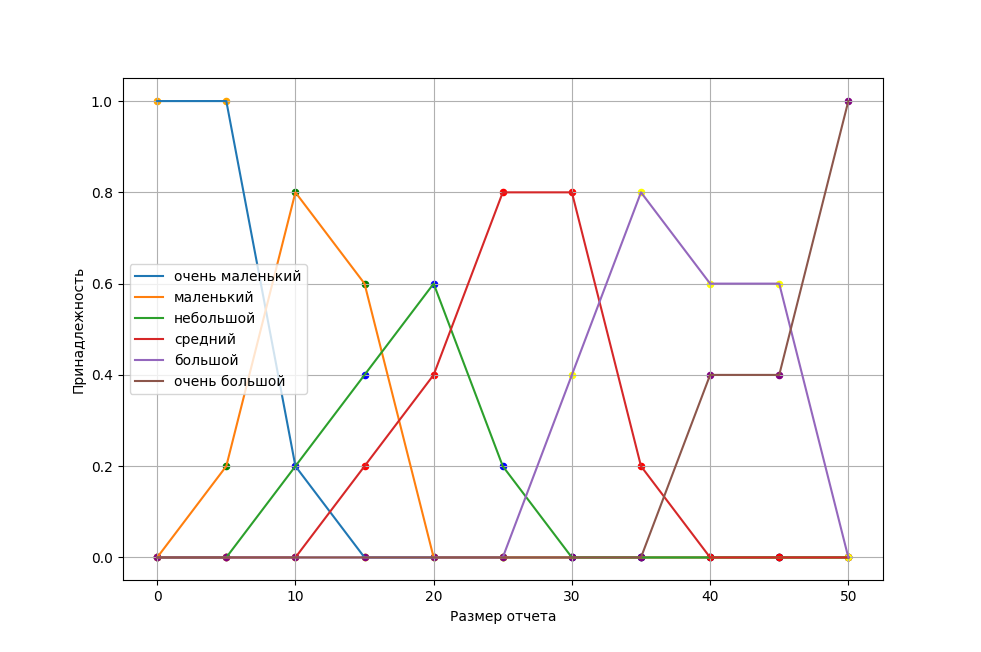
\includegraphics[scale=0.7]{img/graph.png}
            \caption{Функция принадлежности для лингвистической переменной «размер отчета по Анализу алгоритмов»}
            \label{graph:func:1}
        \end{figure}
        \newpage
    \par Исходя из рисунка \ref{graph:func:1} термы относятся к интервалам как:
    \begin{enumerate}
        \item «очень маленький» -- от 0 до 10;
        \item «маленький» -- от 10 до 15;
        \item «небольшой» -- от 15 до 20;
        \item «средний» -- от 20 до 35;
        \item «большой» -- от 35 до 45;
        \item «очень большой» -- от 45 до 50.
    \end{enumerate}

    \section{Требования к ПО}
        Программное обеспечение должно удовлетворять следующим требованиям:
        \begin{itemize}
            \item программа принимает на вход запрос к словарю;
            \item программа выдает массив удовлетволяющих запросу отчетов.
        \end{itemize}
    \section{Средства реализации}
        В качестве языка программирования для реализации данной лабораторной работы был выбран ЯП Python [\ref{bib:5}].
        \par Данный язык достаточно удобен и гибок в использовании.
        \par В качестве среды разработки выбор сделан в сторону Visual Studio Code. Данная среда подходит как для Windows, так и для Linux.

    \section{Листинг программы}
        В приведенном ниже листинге представлена реализация алгоритма полного перебора (листинг \ref{lst:alg:brute}).
        \par \text{           }
        \begin{lstlisting}[language=Python, label=lst:alg:brute, caption=Реализация алгоритма полного перебора]
def find_all(begin, end, not_s = -1, not_e = -1):
    res = []
    for l in data.keys():
        if not_s == -1 and not_e == -1:
            if data.get(l) >= begin and data.get(l) <= end:
                res.append([l,data.get(l)])
        else:
            if data.get(l) >= begin and data.get(l) <= not_s:
                res.append([l,data.get(l)])
            elif data.get(l) >= not_e and data.get(l) <= end:
                res.append([l,data.get(l)])
    return res
\end{lstlisting}

В приведенном ниже листинге представлена реализация алгоритма поиска для каждого терма (листинг \ref{lst:alg:find}).
        \par \text{           }
        \begin{lstlisting}[language=Python, label=lst:alg:find, caption=Реализация алгоритма поиска по термам]
def find_data(request_raz, request_term):

    answer_arrays = []
    for c in request_term:
        if 'не' in c:
            if 'большой' in c:
                answer_arrays.append(find_all(0,50, 35, 45))
            if 'очень большой' in c:
                answer_arrays.append(find_all(0,45))
            if 'средний' in c:
                answer_arrays.append(find_all(0,50,25,35))
            if 'небольшой' in c:
                answer_arrays.append(find_all(0,50, 15,20))
            if 'маленький' in c:
                answer_arrays.append(find_all(0,50, 10,15))
            if 'очень маленький' in c:
                answer_arrays.append(find_all(0,50, 0,10))
        else:
            if 'большой' in c:
                answer_arrays.append(find_all(35, 45))
            if 'очень большой' in c:
                answer_arrays.append(find_all(45,50))
            if 'средний' in c:
                answer_arrays.append(find_all(25,35))
            if 'небольшой' in c:
                answer_arrays.append(find_all(15,20))
            if 'маленький' in c:
                answer_arrays.append(find_all(10,15))
            if 'очень маленький' in c:
                answer_arrays.append(find_all(0,10))
    answer = []
    i = 0
    for raz in request_raz:
        if 'и' in raz and 'или' not in raz:
            if i == 0:
                for a in answer_arrays[i]:
                    if a in answer_arrays[i+1]:
                        answer.append(a)
                i += 2
\end{lstlisting}
        \par \text{           }
        \begin{lstlisting}[language=Python, label=lst:alg:find1, caption=Реализация алгоритма поиска по термам]
            else:
                for a in answer:
                    if a not in answer_arrays[i]:
                        answer.remove(a)
                i+=1
        if 'или' in raz:
            if i == 0:
                for a in answer_arrays[i]:
                    answer.append(a)
                for a in answer_arrays[i+1]:
                    if a not in answer:
                        answer.append(a)
                i += 2
            else:
                for a in answer_arrays[i]:
                    if a not in answer:
                        answer.append(a)
                i+=1
    if len(request_raz) == 0:
        for a in answer_arrays[0]:
            answer.append(a)
    return answer
\end{lstlisting}
    \section{Тестирование ПО}
    Результаты тестирования ПО приведены на рисунках \ref{graph:test:1}, \ref{graph:test:2}, \ref{graph:test:3}.
    
    \begin{figure}[!h]
            \centering
            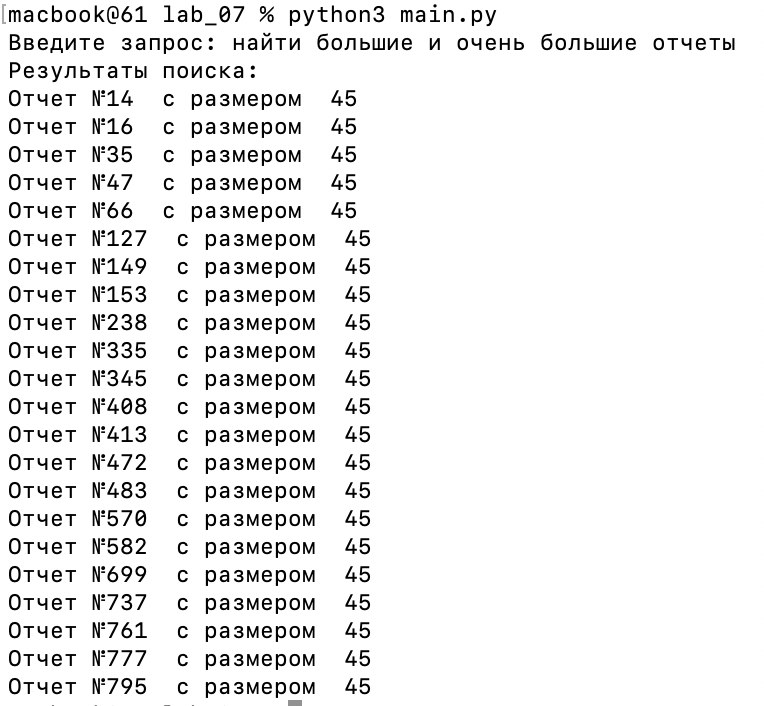
\includegraphics[scale=0.6]{img/2.png}
            \caption{Пример запроса пользователя}
            \label{graph:test:1}
        \end{figure}
        \newpage
    \begin{figure}[!h]
            \centering
            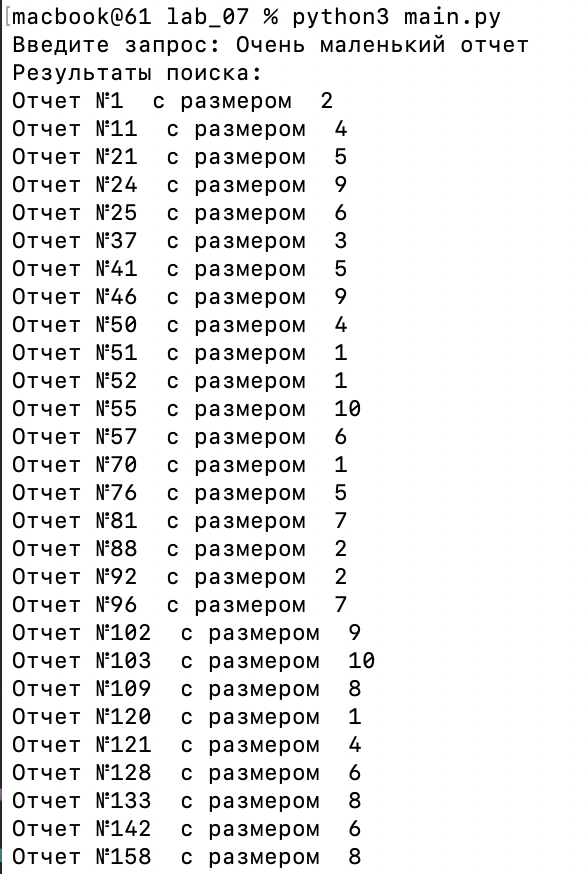
\includegraphics[scale=0.6]{img/1.png}
            \caption{Пример запроса пользователя}
            \label{graph:test:2}
        \end{figure}
\begin{figure}[!h]
            \centering
            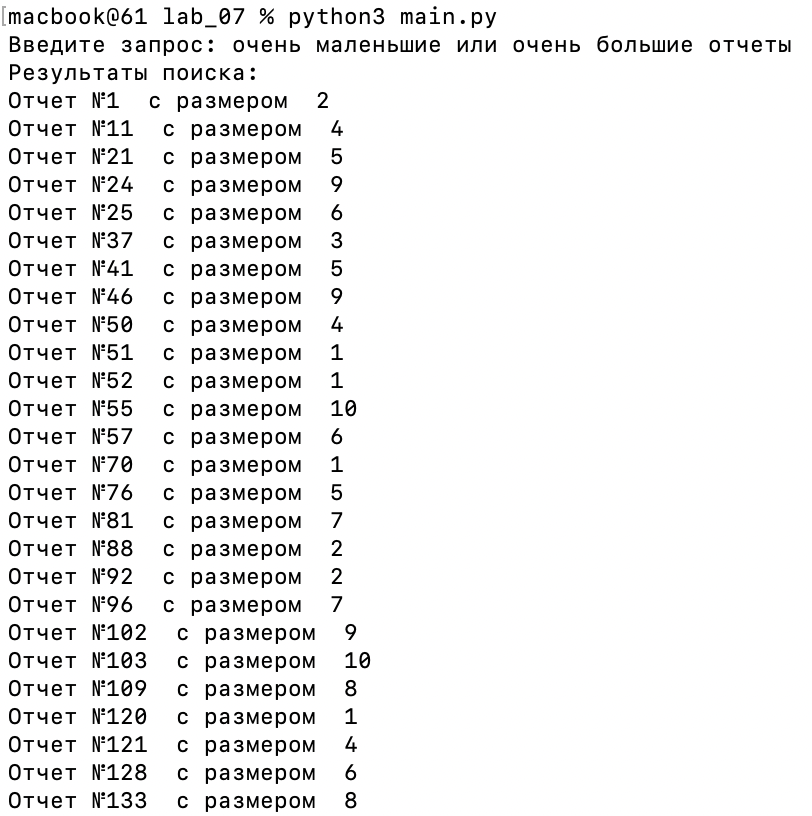
\includegraphics[scale=0.6]{img/3.png}
            \caption{Пример запроса пользователя}
            \label{graph:test:3}
        \end{figure}
        \newpage

    \section*{Вывод}
	
	Было написано и протестировано программное обеспечение для решения поставленной задачи.
    	
\newpage